\chapter{Discussion}

Global Fractal Dimension 
Orion B is more turbulent and we can defo see that 
Orion A double fit -> the changing point is where stars from
We see that point also in the Euler Characteristic
Less so in Orion B, this gives a coherent picture of how the Minkowski functionals can describe the physics of the cloud.

\begin{figure}[t]
    \centering
    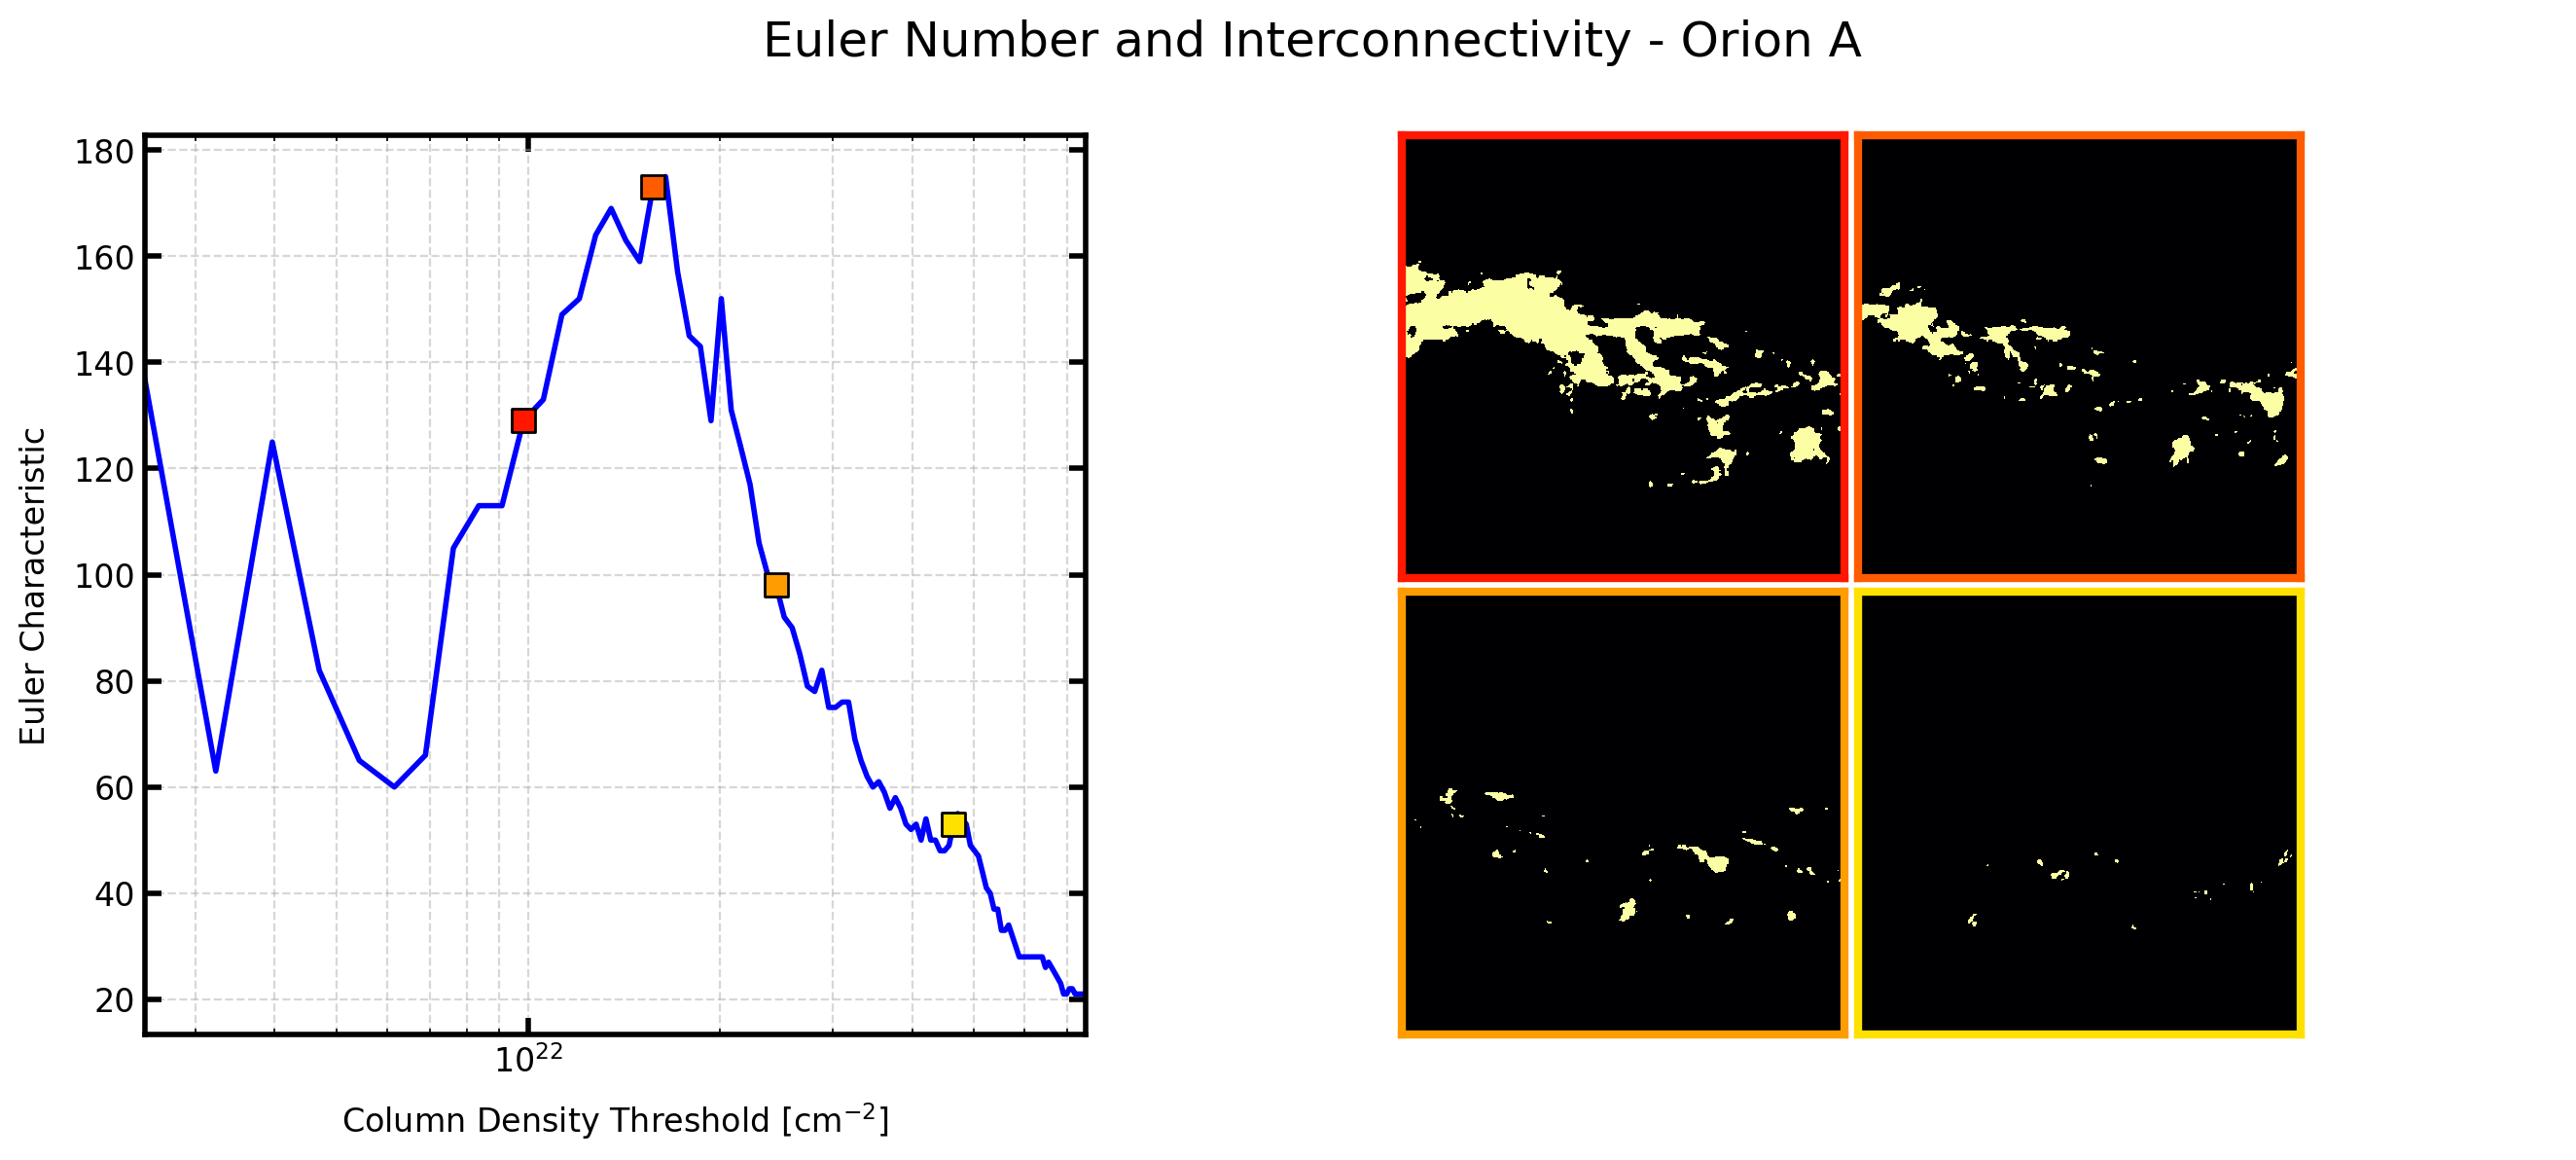
\includegraphics[width=0.6\textwidth]{figures/euler_Orion_A.png}
    \caption{}
    \label{fig:Euler_Orion_A}
\end{figure}

\begin{figure}[t]
    \centering
    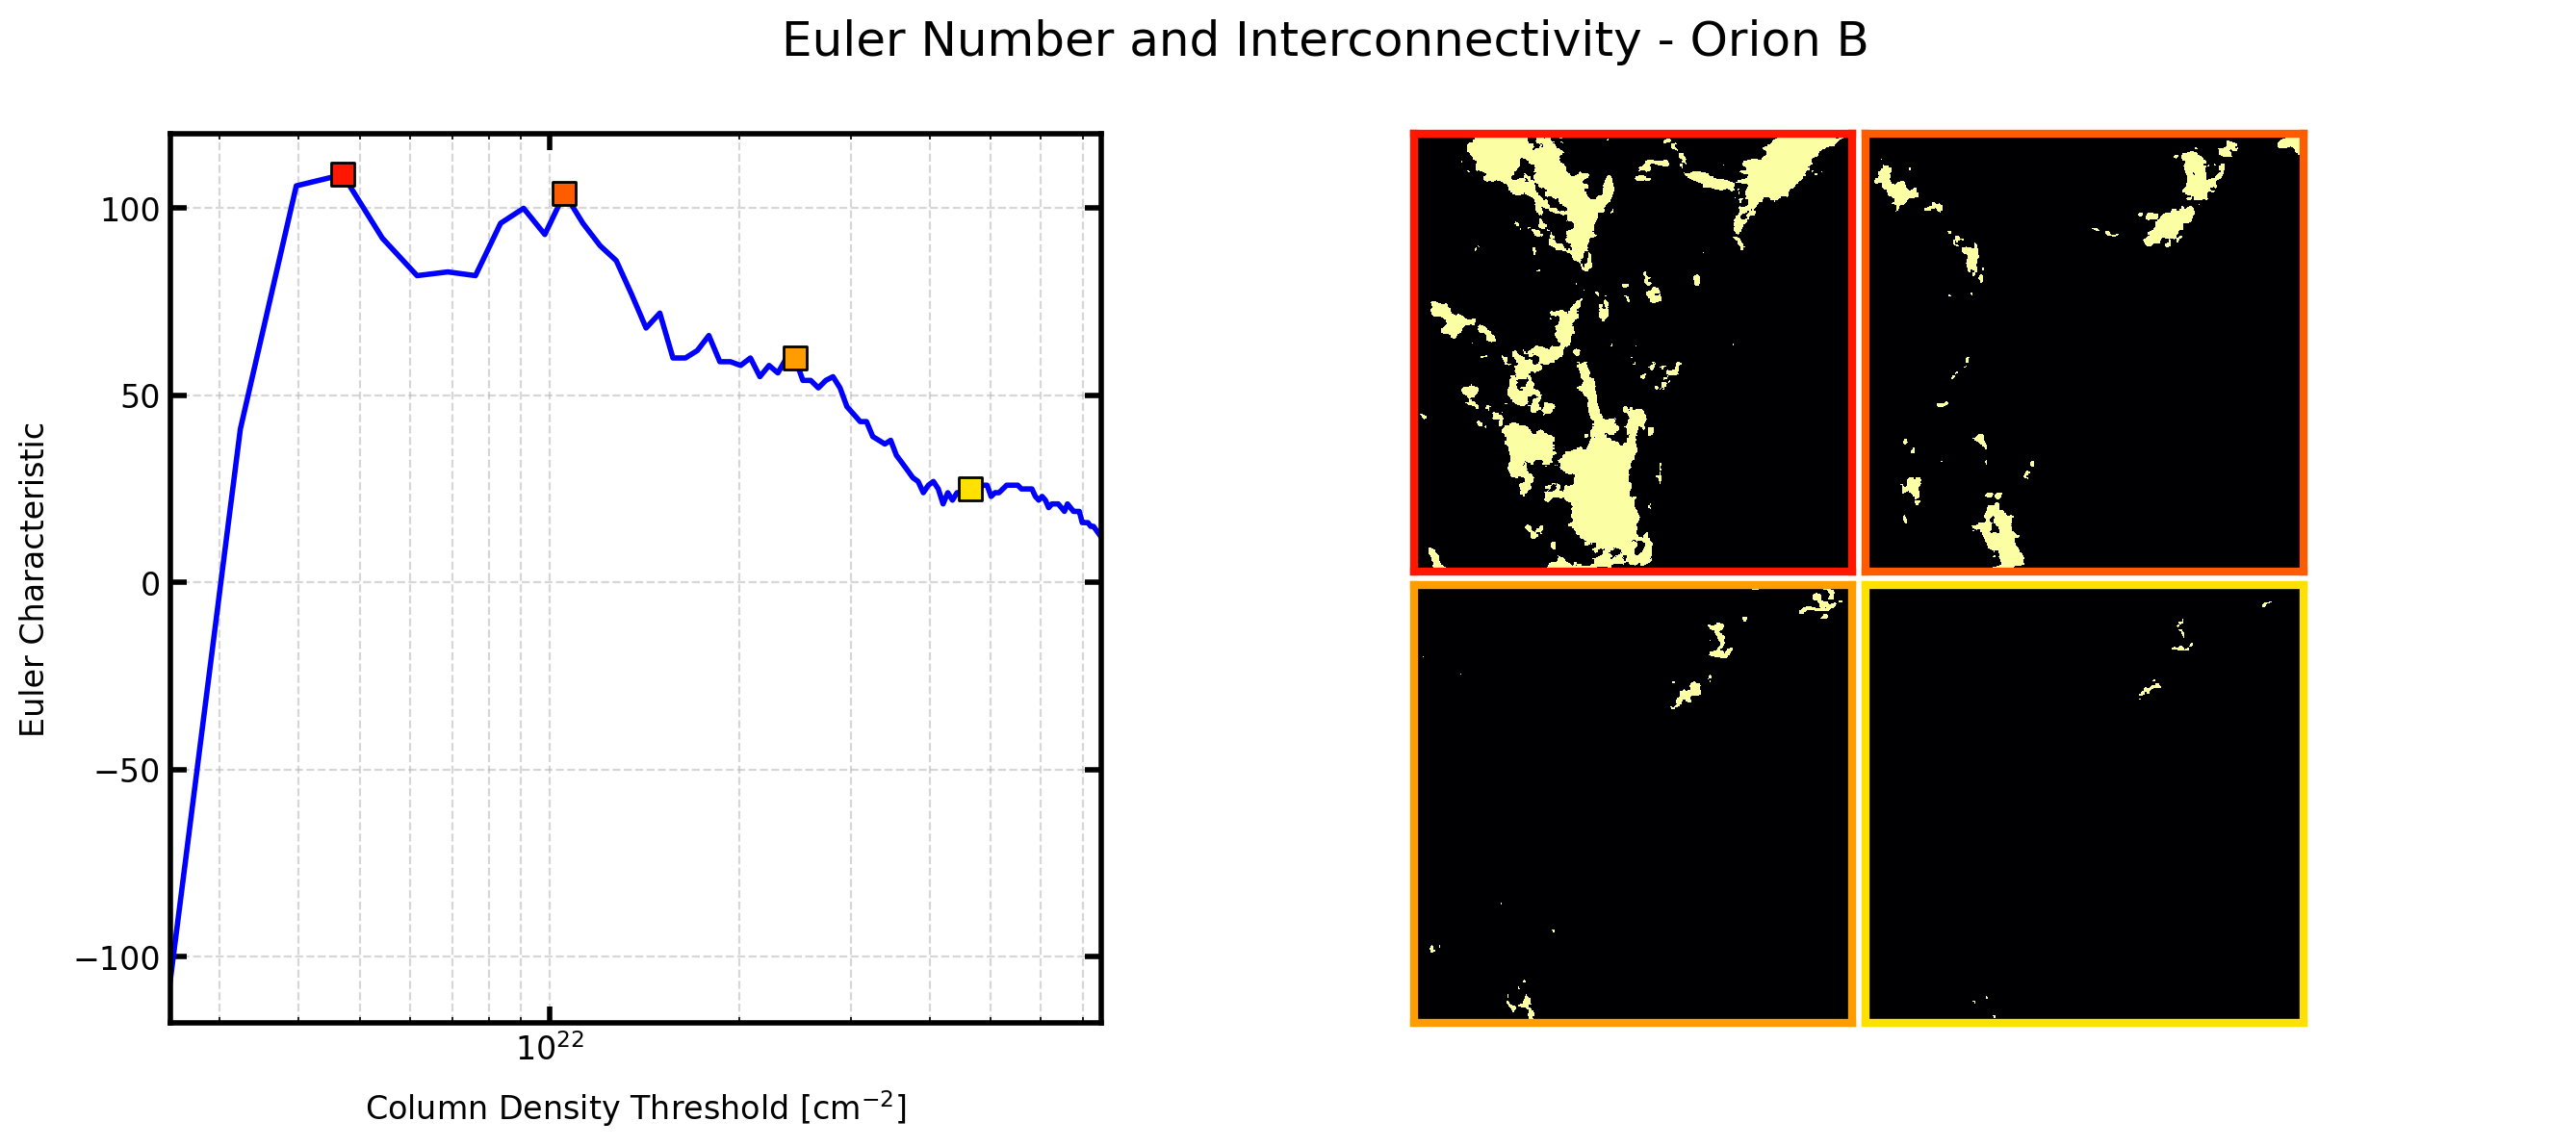
\includegraphics[width=0.6\textwidth]{figures/euler_Orion_B.png}
    \caption{}
    \label{fig:Euler_Orion_B}
\end{figure}

comparison with the M**alpha method

Star Formation: method a bit limited 